%% Issues: One }; missing in bandwidth table by default
%% Same issue appears multiple times in sort table

\def \CILKserialbaseline {3932.2}
\def \CILKblocksize {64}
\def \CILKnumtrials {5}
\def \CILKinputsize {1073741824}
\def \CILKtable {
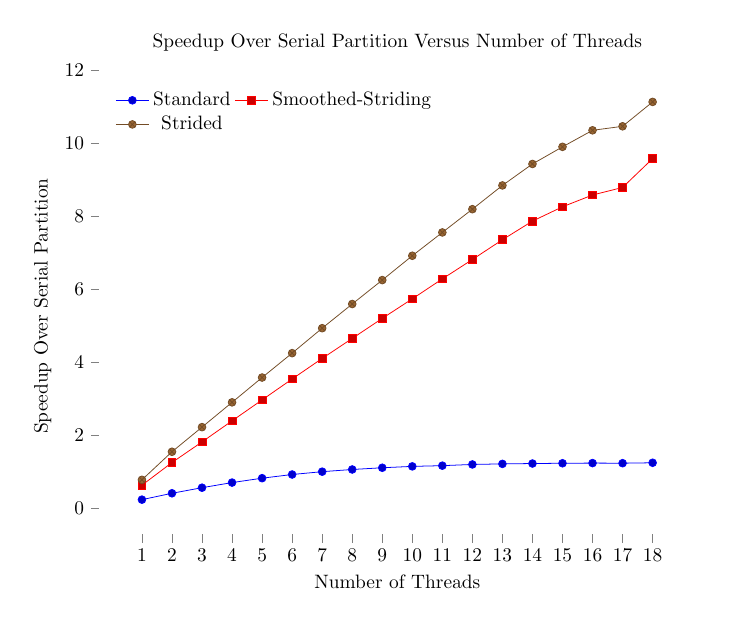
\begin{tikzpicture}[scale = .7]
\begin{axis}[
width = 5 in,
height = 4in,
title={Speedup Over Serial Partition Versus Number of Threads},
xtick pos=left,
ytick pos=left,
legend style={draw=none},
axis line style = { draw = none },
legend pos= north west,
xtick = data,
xlabel={Number of Threads},
ylabel={Speedup Over Serial Partition},
ymax = 12,
legend columns = 2,
scatter/classes=%
{a={mark=o,draw=blue}}]
%% In-Place
% \addplot coordinates {( 1, 0.499048) ( 2, 0.995494) ( 3, 1.42948) ( 4, 1.86113) ( 5, 2.26614) ( 6, 2.65797) ( 7, 2.97174) ( 8, 3.26921) ( 9, 3.43004) ( 10, 3.62281) ( 11, 3.78679) ( 12, 3.89481) ( 13, 4.0002) ( 14, 4.0986) ( 15, 4.15578) ( 16, 4.2191) ( 17, 4.22999) ( 18, 4.27599) };
%% In-Place Prefix-Sum
% \addplot coordinates {( 1, 0.35092) ( 2, 0.636608) ( 3, 0.894292) ( 4, 1.11755) ( 5, 1.32674) ( 6, 1.5096) ( 7, 1.65121) ( 8, 1.77494) ( 9, 1.88432) ( 10, 1.97837) ( 11, 2.0581) ( 12, 2.11591) ( 13, 2.15699) ( 14, 2.18845) ( 15, 2.21159) ( 16, 2.21657) ( 17, 2.20736) ( 18, 2.21557) };
%% Out-of-Place
\addplot coordinates {( 1, 0.223968) ( 2, 0.398625) ( 3, 0.551717) ( 4, 0.691607) ( 5, 0.812203) ( 6, 0.912936) ( 7, 0.990429) ( 8, 1.05055) ( 9, 1.09777) ( 10, 1.13562) ( 11, 1.15517) ( 12, 1.18848) ( 13, 1.20383) ( 14, 1.21364) ( 15, 1.22103) ( 16, 1.22575) ( 17, 1.22285) ( 18, 1.23444) };
%% %% High-Span
%% \addplot coordinates {( 1, 0.796443) ( 2, 1.58021) ( 3, 2.21882) ( 4, 2.93667) ( 5, 3.32899) ( 6, 3.80217) ( 7, 4.3662) ( 8, 4.93375) ( 9, 5.09881) ( 10, 5.42822) ( 11, 5.75051) ( 12, 6.01806) ( 13, 6.37103) ( 14, 6.57999) ( 15, 6.72631) ( 16, 6.95718) ( 17, 7.06722) ( 18, 7.34442) };
%% Cache-Friendly
\addplot coordinates {( 1, 0.619888) ( 2, 1.24099) ( 3, 1.80558) ( 4, 2.38286) ( 5, 2.95654) ( 6, 3.52917) ( 7, 4.09348) ( 8, 4.63922) ( 9, 5.19034) ( 10, 5.72539) ( 11, 6.27145) ( 12, 6.80311) ( 13, 7.34442) ( 14, 7.85497) ( 15, 8.24706) ( 16, 8.57062) ( 17, 8.77723) ( 18, 9.5674) };
%% Strided
\addplot coordinates {( 1, 0.767408) ( 2, 1.5359) ( 3, 2.21084) ( 4, 2.89005) ( 5, 3.56954) ( 6, 4.2382) ( 7, 4.9214) ( 8, 5.58393) ( 9, 6.23961) ( 10, 6.90587) ( 11, 7.54451) ( 12, 8.18186) ( 13, 8.83243) ( 14, 9.4207) ( 15, 9.88984) ( 16, 10.3425) ( 17, 10.4524) ( 18, 11.1205) };
\legend{Standard, Smoothed-Striding, Strided} %% Low-Space, Med-Space, High-Space, Smoothed-Striding, Strided 
\end{axis}
\end{tikzpicture}
}
\def \partitionbandwidthboundserialbaseline {3933.6}
\def \partitionbandwidthboundblocksize {64}
\def \partitionbandwidthboundnumtrials {5}
\def \partitionbandwidthboundinputsize {1073741824}
\def \partitionbandwidthboundtable {
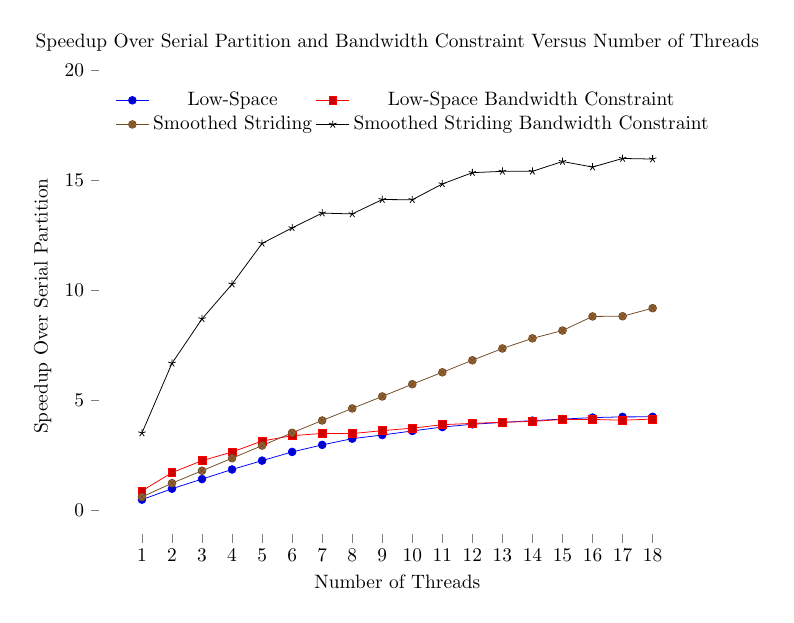
\begin{tikzpicture}[scale = .7]
\begin{axis}[
width = 5 in,
height = 4in,
title={Speedup Over Serial Partition and Bandwidth Constraint Versus Number of Threads},
xtick pos=left,
ytick pos=left,
legend style={draw=none},
axis line style = { draw = none },
legend pos= north west,
xtick = data,
xlabel={Number of Threads},
ylabel={Speedup Over Serial Partition},
ymax = 20,
legend columns = 2,
scatter/classes=%
{a={mark=o,draw=blue}}]
%% In-Place
\addplot coordinates {( 1, 0.499378) ( 2, 0.995949) ( 3, 1.4328) ( 4, 1.86816) ( 5, 2.26982) ( 6, 2.66432) ( 7, 2.98407) ( 8, 3.26602) ( 9, 3.43066) ( 10, 3.61544) ( 11, 3.79325) ( 12, 3.91949) ( 13, 4.00244) ( 14, 4.08389) ( 15, 4.15375) ( 16, 4.22151) ( 17, 4.25438) ( 18, 4.25622) };
%% Low-Space Bandwidth Bound
\addplot coordinates {(1, 0.894939)(2, 1.72634)(3, 2.26699)(4, 2.66131)(5, 3.15777)(6, 3.4024)(7, 3.50312)(8, 3.49686)(9, 3.62955)(10, 3.74294)(11, 3.90093)(12, 3.9593)(13, 4.0131)(14, 4.04714)(15, 4.13799)(16, 4.13782)(17, 4.10515)(18, 4.15355)};
%% high span
%% \addplot coordinates {( 1, 0.812828) ( 2, 1.61997) ( 3, 2.22137) ( 4, 2.95626) ( 5, 3.33582) ( 6, 3.80352) ( 7, 4.36001) ( 8, 5.10062) ( 9, 5.11521) ( 10, 5.44217) ( 11, 5.74752) ( 12, 6.07787) ( 13, 6.41278) ( 14, 6.63787) ( 15, 6.68752) ( 16, 6.79848) ( 17, 7.10549) ( 18, 7.26292) };
%% %% High-Span Bandwidth Bound
%% \addplot coordinates {(1, 1.75849)(2, 3.34185)(3, 4.35383)(4, 5.15739)(5, 5.9788)(6, 6.31621)(7, 6.76074)(8, 6.76348)(9, 6.99773)(10, 7.10173)(11, 7.39957)(12, 7.51437)(13, 7.7436)(14, 7.76191)(15, 7.89966)(16, 7.87403)(17, 7.94484)(18, 8.05483)}; %% cache friendly
\addplot coordinates {( 1, 0.62101) ( 2, 1.24639) ( 3, 1.81072) ( 4, 2.37852) ( 5, 2.95182) ( 6, 3.53233) ( 7, 4.09153) ( 8, 4.63759) ( 9, 5.18124) ( 10, 5.73746) ( 11, 6.27769) ( 12, 6.82206) ( 13, 7.35802) ( 14, 7.81717) ( 15, 8.17117) ( 16, 8.81183) ( 17, 8.81973) ( 18, 9.18636) };
%% Cache-Friendly Bandwidth Bound
\addplot coordinates {(1, 3.52223)(2, 6.68603)(3, 8.70095)(4, 10.276)(5, 12.1258)(6, 12.8292)(7, 13.4991)(8, 13.4622)(9, 14.1134)(10, 14.1066)(11, 14.8215)(12, 15.3338)(13, 15.3938)(14, 15.3942)(15, 15.8412)(16, 15.5877)(17, 15.9778)(18, 15.9519)};
\legend{Low-Space, Low-Space Bandwidth Constraint, Smoothed Striding, Smoothed Striding Bandwidth Constraint}
\end{axis}
\end{tikzpicture}
}

\def \CILKsortblocksize {64}
\def \CILKsortnumtrials {5}
\def \CILKsortmaxinputsize {1073741824}
\def \CILKsorttable {
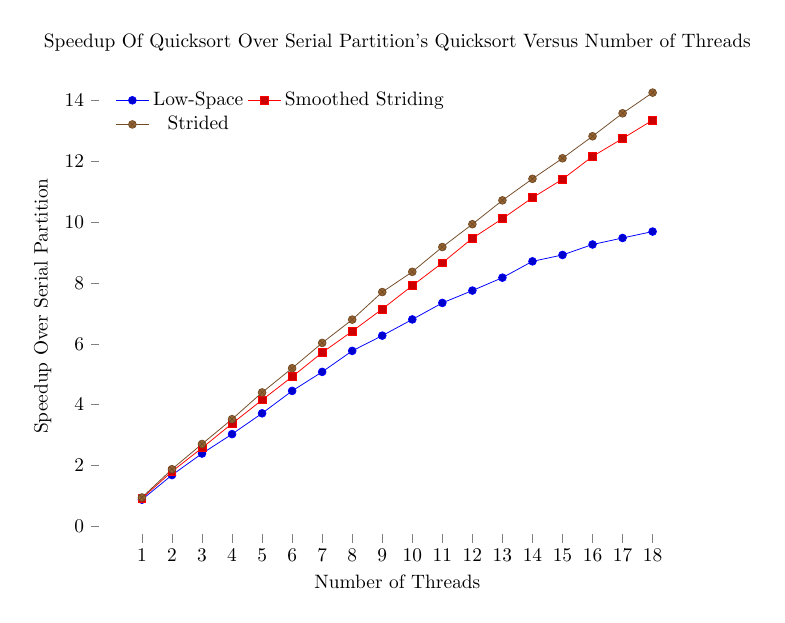
\begin{tikzpicture}[scale = .7]
\begin{axis}[
width = 5 in,
height = 4in,
title={Speedup Of Quicksort Over Serial Partition's Quicksort Versus Number of Threads},
xtick pos=left,
ytick pos=left,
legend style={draw=none},
axis line style = { draw = none },
legend pos= north west,
xtick = data,
xlabel={Number of Threads},
ylabel={Speedup Over Serial Partition},
ymax = 15,
legend columns = 2,
scatter/classes=%
{a={mark=o,draw=blue}}]
%% %% Low Space with log size 24
%% \addplot coordinates {( 1, 0.863202) ( 2, 1.63232) ( 3, 2.29705) ( 4, 2.96413) ( 5, 3.59298) ( 6, 4.1696) ( 7, 4.71085) ( 8, 5.2279) ( 9, 5.8474) ( 10, 6.4043) ( 11, 6.55736) ( 12, 7.21241) ( 13, 7.57064) ( 14, 7.99417) ( 15, 8.4679) ( 16, 8.93099) ( 17, 9.04881) ( 18, 9.60644) %% High-Span with log size 24
%% \addplot coordinates {( 1, 0.960106) ( 2, 1.88538) ( 3, 2.72075) ( 4, 3.47467) ( 5, 4.2576) ( 6, 5.08451) ( 7, 5.93339) ( 8, 6.47686) ( 9, 7.1822) ( 10, 7.57901) ( 11, 8.44704) ( 12, 8.64943) ( 13, 9.16979) ( 14, 9.04881) ( 15, 10.1464) ( 16, 9.61992) ( 17, 10.5199) ( 18, 9.38304) %% Cache Friendly with log size 24
%% \addplot coordinates {( 1, 0.900013) ( 2, 1.74752) ( 3, 2.46372) ( 4, 3.23233) ( 5, 3.90159) ( 6, 4.62508) ( 7, 5.46099) ( 8, 6.15157) ( 9, 6.85215) ( 10, 7.53736) ( 11, 8.11716) ( 12, 8.74872) ( 13, 9.70156) ( 14, 9.04881) ( 15, 11.0273) ( 16, 10.87) ( 17, 12.1829) ( 18, 12.2482) %% Strided with log size 24
%% \addplot coordinates {( 1, 0.95079) ( 2, 1.82955) ( 3, 2.63808) ( 4, 3.45716) ( 5, 4.20798) ( 6, 4.99199) ( 7, 5.78819) ( 8, 6.56364) ( 9, 7.37527) ( 10, 8.03162) ( 11, 8.89624) ( 12, 9.61992) ( 13, 9.7153) ( 14, 11.1167) ( 15, 10.9394) ( 16, 11.4891) ( 17, 13.1651) ( 18, 13.9695) };
%% %% Low Space with log size 26
%% \addplot coordinates {( 1, 0.861043) ( 2, 1.63325) ( 3, 2.3004) ( 4, 2.98343) ( 5, 3.63316) ( 6, 4.19898) ( 7, 4.82886) ( 8, 5.34581) ( 9, 5.89992) ( 10, 6.44372) ( 11, 6.94206) ( 12, 7.4672) ( 13, 7.60676) ( 14, 8.0564) ( 15, 8.64475) ( 16, 8.82709) ( 17, 8.76202) ( 18, 8.96831) %% High-Span with log size 26
%% \addplot coordinates {( 1, 0.955523) ( 2, 1.86586) ( 3, 2.6845) ( 4, 3.49224) ( 5, 4.27081) ( 6, 5.0929) ( 7, 5.83274) ( 8, 6.53586) ( 9, 7.29308) ( 10, 7.90003) ( 11, 8.63721) ( 12, 8.97915) ( 13, 9.7769) ( 14, 10.1893) ( 15, 10.5812) ( 16, 10.7887) ( 17, 10.7613) ( 18, 10.3418) %% Cache Friendly with log size 26
%% \addplot coordinates {( 1, 0.914609) ( 2, 1.73339) ( 3, 2.49178) ( 4, 3.22151) ( 5, 4.02384) ( 6, 4.70946) ( 7, 5.57239) ( 8, 6.13884) ( 9, 6.93881) ( 10, 7.59315) ( 11, 8.23047) ( 12, 8.91717) ( 13, 9.42939) ( 14, 10.1302) ( 15, 10.6801) ( 16, 10.8359) ( 17, 11.3883) ( 18, 11.3189) %% Strided with log size 26
%% \addplot coordinates {( 1, 0.946785) ( 2, 1.82922) ( 3, 2.64766) ( 4, 3.4262) ( 5, 4.2788) ( 6, 5.08245) ( 7, 5.95192) ( 8, 6.67986) ( 9, 7.44475) ( 10, 8.25563) ( 11, 8.94132) ( 12, 9.74164) ( 13, 10.4362) ( 14, 11.3621) ( 15, 11.4851) ( 16, 12.2071) ( 17, 12.6542) ( 18, 13.4993) };
%% %% Low Space with log size 28
%% \addplot coordinates {( 1, 0.862267) ( 2, 1.63941) ( 3, 2.34664) ( 4, 2.96157) ( 5, 3.64611) ( 6, 4.31258) ( 7, 4.88345) ( 8, 5.43042) ( 9, 5.87762) ( 10, 6.44029) ( 11, 7.00878) ( 12, 7.30452) ( 13, 7.83539) ( 14, 8.12956) ( 15, 8.50856) ( 16, 8.76302) ( 17, 8.98741) ( 18, 9.33821) %% High-Span with log size 28
%% \addplot coordinates {( 1, 0.939362) ( 2, 1.84744) ( 3, 2.6917) ( 4, 3.45716) ( 5, 4.29244) ( 6, 5.08279) ( 7, 5.79208) ( 8, 6.6353) ( 9, 7.2093) ( 10, 8.01682) ( 11, 8.74742) ( 12, 9.17326) ( 13, 9.7479) ( 14, 10.2979) ( 15, 11.0745) ( 16, 11.4344) ( 17, 11.4888) ( 18, 12.34) %% Cache Friendly with log size 28
%% \addplot coordinates {( 1, 0.908881) ( 2, 1.75263) ( 3, 2.51771) ( 4, 3.28228) ( 5, 4.01042) ( 6, 4.74982) ( 7, 5.54834) ( 8, 6.2393) ( 9, 6.98884) ( 10, 7.70125) ( 11, 8.41219) ( 12, 9.06778) ( 13, 9.67555) ( 14, 10.3505) ( 15, 11.0125) ( 16, 11.4744) ( 17, 12.1533) ( 18, 12.4095) %% Strided with log size 28
%% \addplot coordinates {( 1, 0.942529) ( 2, 1.82563) ( 3, 2.6044) ( 4, 3.46053) ( 5, 4.25683) ( 6, 5.12315) ( 7, 5.88602) ( 8, 6.70811) ( 9, 7.43113) ( 10, 8.17952) ( 11, 8.96974) ( 12, 9.68435) ( 13, 10.4214) ( 14, 10.9587) ( 15, 11.71) ( 16, 12.2949) ( 17, 12.9046) ( 18, 13.3107) };
%% Low Space with log size 30
\addplot coordinates {( 1, 0.87864) ( 2, 1.68661) ( 3, 2.39404) ( 4, 3.03172) ( 5, 3.71549) ( 6, 4.45118) ( 7, 5.07595) ( 8, 5.76618) ( 9, 6.26716) ( 10, 6.79929) ( 11, 7.34223) ( 12, 7.74736) ( 13, 8.17148) ( 14, 8.70784) ( 15, 8.91736) ( 16, 9.26139) ( 17, 9.47532) ( 18, 9.68665)}; %% High-Span with log size 30
%% \addplot coordinates {( 1, 0.96225) ( 2, 1.879) ( 3, 2.71741) ( 4, 3.56118) ( 5, 4.44821) ( 6, 5.29223) ( 7, 5.97895) ( 8, 6.76091) ( 9, 7.59373) ( 10, 8.37912) ( 11, 9.01587) ( 12, 9.58729) ( 13, 10.1906) ( 14, 10.881) ( 15, 11.4166) ( 16, 12.026) ( 17, 12.3279) ( 18, 12.6408)}; %% Cache Friendly with log size 30
\addplot coordinates {( 1, 0.921182) ( 2, 1.80562) ( 3, 2.57745) ( 4, 3.37831) ( 5, 4.15358) ( 6, 4.91613) ( 7, 5.7093) ( 8, 6.41041) ( 9, 7.14098) ( 10, 7.907) ( 11, 8.6573) ( 12, 9.46479) ( 13, 10.1098) ( 14, 10.7975) ( 15, 11.4046) ( 16, 12.1549) ( 17, 12.7427) ( 18, 13.346)}; %% Strided with log size 30
\addplot coordinates {( 1, 0.949951) ( 2, 1.87888) ( 3, 2.70758) ( 4, 3.52248) ( 5, 4.40049) ( 6, 5.19675) ( 7, 6.02708) ( 8, 6.79362) ( 9, 7.69896) ( 10, 8.36354) ( 11, 9.17828) ( 12, 9.92823) ( 13, 10.7114) ( 14, 11.4187) ( 15, 12.0935) ( 16, 12.8171) ( 17, 13.5719) ( 18, 14.2507) };
\legend{Low-Space, Smoothed Striding, Strided}
\end{axis}
\end{tikzpicture}
}

%% Bandwith results without numactl:
%% \def \partitionbandwidthboundserialbaseline {3832}
%% \def \partitionbandwidthboundblocksize {64}
%% \def \partitionbandwidthboundnumtrials {5}
%% \def \partitionbandwidthboundinputsize {1073741824}
%% \def \partitionbandwidthboundtable {
%% \begin{tikzpicture}[scale = .8]
%% \begin{axis}[
%% width = 5 in,
%% height = 4in,
%% title={Speedup Versus Number of Threads},
%% xtick pos=left,
%% ytick pos=left,
%% legend style={draw=none},
%% axis line style = { draw = none },
%% legend pos= north west,
%% xtick = data,
%% xlabel={Number of Threads},
%% ylabel={Speedup Over Serial Partition},
%% ymax = 4,
%% legend columns = 2,
%% scatter/classes=%
%% {a={mark=o,draw=blue}}]
%% %% In-Place
%% \addplot coordinates {( 1, 0.504928) ( 2, 0.744917) ( 3, 1.27793) ( 4, 1.62967) ( 5, 1.91677) ( 6, 2.3244) ( 7, 2.47865) ( 8, 2.58186) ( 9, 2.68573) ( 10, 2.78448) ( 11, 2.7756) ( 12, 2.85077) ( 13, 2.86826) ( 14, 2.91407) ( 15, 2.90479) ( 16, 2.94769) ( 17, 2.95497) ( 18, 2.94588) };
%% %% Low-Space Bandwidth Bound
%% \addplot coordinates {(1, 1.05385)(2, 1.63936)(3, 1.81183)(4, 2.05614)(5, 2.39067)(6, 2.5237)(7, 2.40513)(8, 2.55015)(9, 2.58884)(10, 2.57444)(11, 2.69167)(12, 2.66946)(13, 2.64859)(14, 2.68175)(15, 2.66023)(16, 2.69318)(17, 2.68783)(18, 2.72913)};
%% %% high span
%% \addplot coordinates {( 1, 0.816814) ( 2, 1.47691) ( 3, 1.98529) ( 4, 2.63875) ( 5, 3.01305) ( 6, 3.40441) ( 7, 3.68887) ( 8, 3.97345) ( 9, 4.14181) ( 10, 4.27297) ( 11, 4.46724) ( 12, 4.45271) ( 13, 4.45271) ( 14, 4.62355) ( 15, 4.60024) ( 16, 4.70184) ( 17, 4.55431) ( 18, 4.71225) };
%% %% High-Span Bandwidth Bound
%% \addplot coordinates {(1, 2.03744)(2, 3.14521)(3, 3.47353)(4, 3.91661)(5, 4.536)(6, 4.70395)(7, 4.47075)(8, 4.76355)(9, 4.86065)(10, 4.68934)(11, 4.86418)(12, 4.98468)(13, 4.9239)(14, 4.99117)(15, 4.94174)(16, 4.98761)(17, 4.96382)(18, 5.00564)%% cache friendly
%% \addplot coordinates {( 1, 0.621291) ( 2, 1.06581) ( 3, 1.76541) ( 4, 2.28204) ( 5, 2.8838) ( 6, 3.49253) ( 7, 4.04561) ( 8, 4.56843) ( 9, 4.97921) ( 10, 5.6089) ( 11, 5.8791) ( 12, 6.26963) ( 13, 6.8331) ( 14, 6.87971) ( 15, 7.15459) ( 16, 7.38343) ( 17, 8.25151) ( 18, 8.35587) };
%% %% Cache-Friendly Bandwidth Bound
%% \addplot coordinates {(1, 4.06363)(2, 6.29023)(3, 6.9299)(4, 7.88794)(5, 9.08502)(6, 9.329)(7, 9.45987)(8, 9.53406)(9, 9.91163)(10, 9.90729)(11, 9.70433)(12, 10.1146)(13, 9.9126)(14, 9.85886)(15, 9.86993)(16, 10.0183)(17, 10.0765)(18, 9.99261)};
%% \legend{Low-Space, Low-Space Bandwidth Constraint, Two-Layer, Two-Layer Bandwidth Constraint}
%% \end{axis}
%% \end{tikzpicture}
%% }
